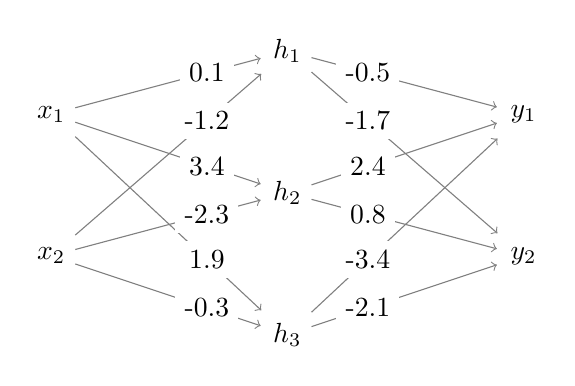
\begin{tikzpicture}[shorten >=1pt,->,draw=black!50, node distance=\layersep]
    \def\layersep{3cm}
    \def\ysep{1.8}
    \tikzstyle{every pin edge}=[<-,shorten <=1pt]
    \tikzstyle{neuron}=[minimum size=17pt,inner sep=0pt]
    \tikzstyle{input neuron}=[neuron];
    \tikzstyle{output neuron}=[neuron];
    \tikzstyle{hidden neuron}=[neuron];
    \tikzstyle{annot} = [text width=4em, text centered]

    % Draw the input layer nodes
    \foreach \y in {1,...,2}
        \node[input neuron] (I-\y) at (0,-\ysep*\y) {$x_\y$};

    % Draw the hidden layer nodes
    \foreach \y in {1,...,3}
        \path[yshift=0.8cm]
            node[hidden neuron] (H-\y) at (\layersep,-\ysep*\y cm) {$h_\y$};

    % Draw the output layer node
    \foreach \y in {1,...,2}
        \node[output neuron] (O-\y) at (2*\layersep,-\ysep*\y cm) {$y_\y$};

    \def\xhweights{{{0.1,3.4,1.9},{-1.2,-2.3,-0.3}}}
    % Connect every node in the input layer with every node in the
    % hidden layer.
    \foreach \source in {1,...,2}
        \foreach \dest in {1,...,3}
            \pgfmathsetmacro{\sourceminus}{int(\source-1)}
            \pgfmathsetmacro{\destminus}{int(\dest-1)}
            \draw (I-\source) -> (H-\dest) node[pos=.7,fill=white] {
                \pgfmathparse{\xhweights[\sourceminus][\destminus]}%
                \pgfmathresult
            };

    \def\hyweights{{{-0.5,-1.7},{2.4,0.8},{-3.4,-2.1}}}
    % Connect every node in the hidden layer with the output layer
    \foreach \source in {1,...,3}
        \foreach \dest in {1,...,2}
            \pgfmathsetmacro{\sourceminus}{int(\source-1)}
            \pgfmathsetmacro{\destminus}{int(\dest-1)}
            \draw (H-\source) -> (O-\dest) node[pos=.3,fill=white] {
                \pgfmathparse{\hyweights[\sourceminus][\destminus]}%
                \pgfmathresult
            };
\end{tikzpicture}